\documentclass[UTF8]{article} % Default font size is 12pt, it can be changed here ctexart

\usepackage{geometry} % Required to change the page size to A4
\geometry{a4paper} % Set the page size to be A4 as opposed to the default US Letter
\geometry{left=1.6cm,right=1.6cm,top=3.5cm,bottom=3.5cm}
\usepackage{subfigure}
\usepackage{graphicx} % Required for including pictures
\usepackage{amsmath}
\usepackage{amssymb,bm}
\usepackage{float} % Allows putting an [H] in \begin{figure} to specify the exact location of the figure
%\usepackage{wrapfig} % Allows in-line images such as the example fish picture

%\linespread{1.2} % Line spacing

%\setlength\parindent{0pt} % Uncomment to remove all indentation from paragraphs

\graphicspath{{Pictures/}} % Specifies the directory where pictures are stored

\begin{document}

%----------------------------------------------------------------------------------------
%	TITLE PAGE
%----------------------------------------------------------------------------------------

\begin{titlepage}

\newcommand{\HRule}{\rule{\linewidth}{0.5mm}} % Defines a new command for the horizontal lines, change thickness here

\center % Center everything on the page
%%\includegraphics[width=2.5cm]{Pictures/SCE.png}
%%\textsc{\LARGE University Name}\\[1.5cm] % Name of your university/college
%%\textsc{\Large Major Heading}\\[0.5cm] % Major heading such as course name
%%\textsc{\large Minor Heading}\\[0.5cm] % Minor heading such as course title

\HRule \\[0.4cm]
{ \huge \bfseries Statistics}\\[0.4cm] % Title of your document
\HRule \\[1.5cm]

\begin{minipage}{0.4\textwidth}
\begin{flushleft} \large
\emph{Author:}\\
Ming \textsc{Li} % Your name
\end{flushleft}
\end{minipage}
~
\begin{minipage}{0.4\textwidth}
\begin{flushright} \large
\emph{Department:} \\
Mathematics
\end{flushright}
\end{minipage}\\[4cm]

{\large \today}\\[3cm] % Date, change the \today to a set date if you want to be precise

%\includegraphics{Logo}\\[1cm] % Include a department/university logo - this will require the graphicx package

\vfill % Fill the rest of the page with whitespace
\end{titlepage}
\newpage
\section{Introduction}
The probability theory mainly research random variables such as $x$. $x$ could be some of the values with a measure call probability:
$$
P(x=k),\quad P(x \in A), \quad\text{where}\quad A \quad\text{is a Boreal set}
$$
The general study of statistics is to find out the distribution of $x$, hopefully, the probability distribution function or cumulative distribution function. Moreover, for multivariate variables, the task could be to find out the joint distribution($P(x_1,x_2,\vdots)$) or conditional distribution($P(x|y)$). Typically, the following steps:
\begin{itemize}
\item Guess what should be the right distribution
\item Estimate the parameters
\item Prove your suppose(prove the distribution assumption or the parameters estimation is right)
\end{itemize}
So, this document is going to review the basic points of statistics follow the step: guess$\rightarrow$estimate$\rightarrow$prove.

\section{Guess}
\subsection{Data perspective}
Normally, the histogram chart can help us for a general perspective of the data probability distribution (data.hist(grid=...)) or cumulative distribution (idate.plot.hist(cumulative=True)).
\begin{figure}[htb]
\centering
\subfigure[probability distribution]{
\label{Fig.sub.1}
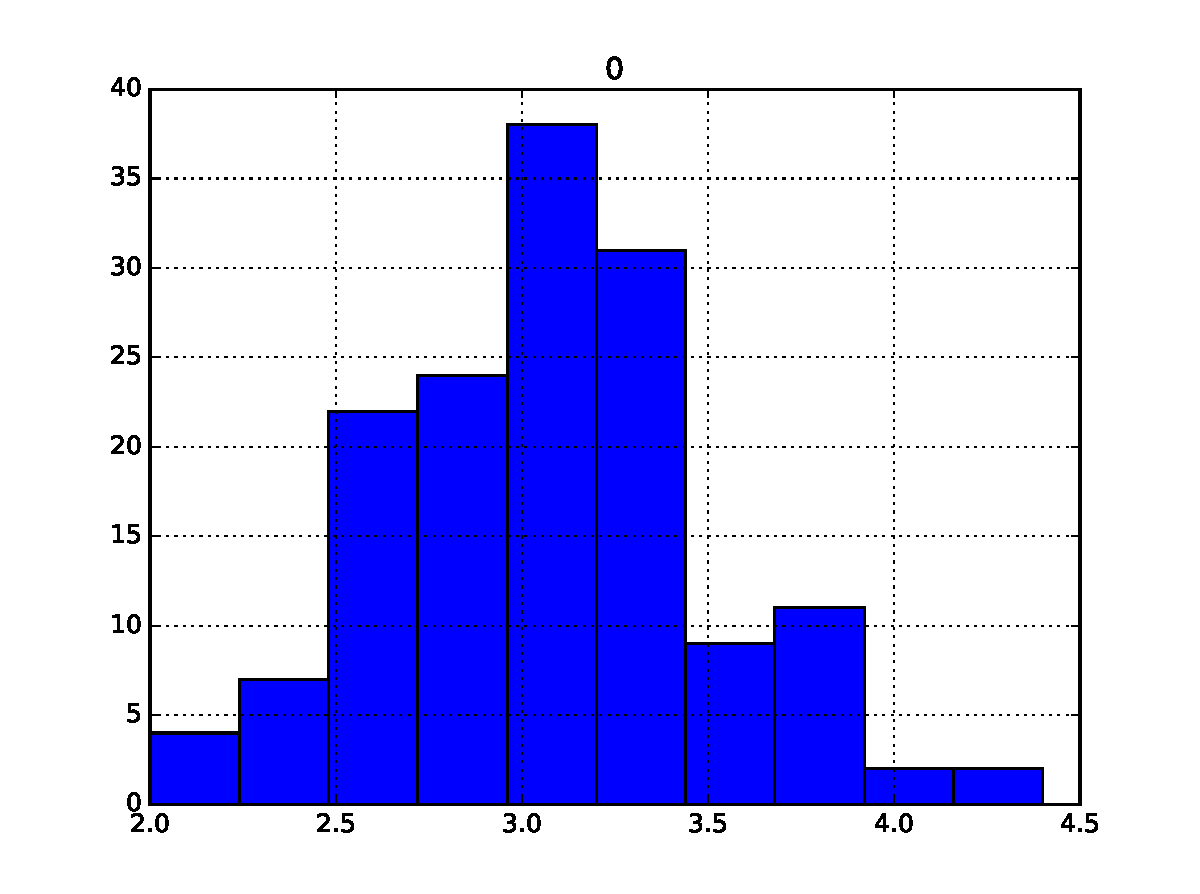
\includegraphics[height=6cm,width=8cm]{pic/hist.pdf}}
\subfigure[cumulative distribution]{
\label{Fig.sub.2}
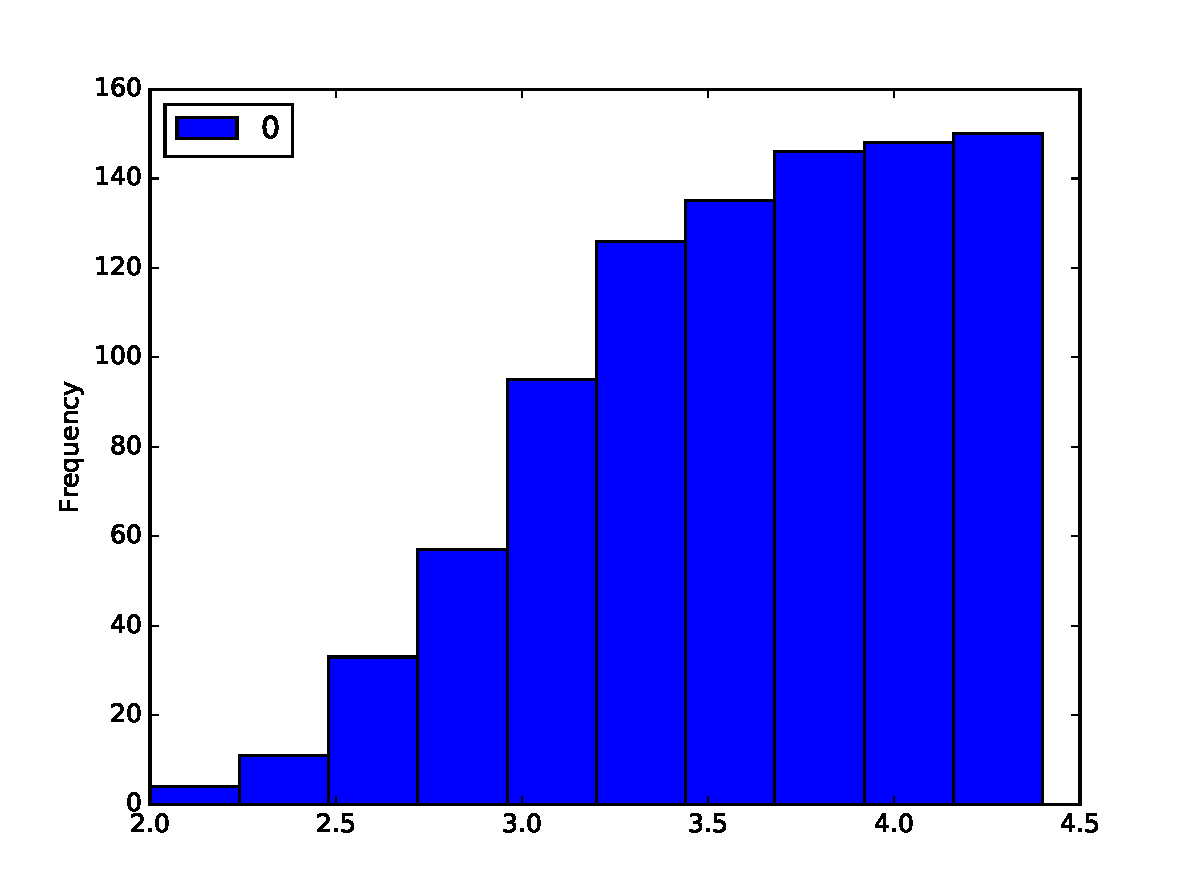
\includegraphics[height=6cm,width=8cm]{pic/cumulative.pdf}}
\caption{Histogram}
\label{fig:2}
\end{figure}
\subsection{Type of distributions}




And the estimation of probability distribution
$$
P(s_k<x\leq s_{k+1})\approx \sum I(s_k<x_i\leq s_{k+1})/N
$$
or cumulative distribution
$$
P(x\leq s_{k+1})\approx\sum I(x_i\leq s_{k+1})/N
$$


\section{Estimate}

\section{Prove}




\end{document}
